\documentclass[10pt,a4paper]{article}
\usepackage[utf8]{inputenc}
\usepackage[T1]{fontenc}
\usepackage{fullpage}
\usepackage{amsfonts,amsmath,amssymb,mathtools, bm}
\usepackage{comment,color, fancybox}
\usepackage{verbatim}
\usepackage{enumitem}
\usepackage{listings}
\usepackage{xcolor}
\usepackage{array}
\usepackage{ragged2e}
\usepackage{csvsimple}
\usepackage{changepage}
% \usepackage[alf]{ABNTex/abntex2cite}
\usepackage[ddmmyyyy]{datetime}

\lstset{basicstyle=\ttfamily,
	showstringspaces=false,
	commentstyle=\color{red},
	keywordstyle=\color{blue}
}

\newcommand{\ttt}[1]{\texttt{#1}}

\title{Relatório do Desempenho de Aplicações Paralelas} 
\author{Miguel Nunes}
\date{\today}

\begin{document}
	\maketitle

	\section{Algoritmos e Descrição do Ambiente}

		Foram analisados os algoritmos de Mandelbrot e Multiplicação de Matrizes, com apenas leves modificações na entrada de dados para
		facilitar a automatização dos testes.
		Para o algoritmo de Mandelbrot, foram utilizadas os valores: 
		
		\begin{verbatim}
			max_row    = 340
			max_column = 1000
			max_n      = 4600
		\end{verbatim}

		Pois foi observado experimentalmente que, em execuções sequenciais do algoritmo, essas entradas levavam, em média, 
		64 segundos para serem processadas.

		Já para o algoritmo de Multiplicação de Matrizes, a entrada \texttt{n = 2340} foi utilizada, pois, 
		análogo ao caso anterior, foi observado que essa entrada levava, em média, 54 segundos para ser processada.

		Os testes foram realizados num computador com as seguintes especificações:

		\begin{description}
			\item[CPU] \texttt{AMD Ryzen 7 5700G with Radeon Graphics (16) @ 4.673GH}
			\item[Memória] \texttt{63588MiB}
			\item[OS] \texttt{Fedora Linux 36 (MATE-Compiz) x86\_64}
			\item[Kernel] \texttt{5.18.19-200.fc36.x86\_64}
		\end{description}

		Os testes foram executados automaticamente a partir de um script em bash, com o auxílio de um makefile. As entradas para os 
		testes eram geradas pelo makefile, ao início de uma nova rodada de testes, todos os arquivos gerados no teste anterior são deletados.

	\section{Coleta dos Dados}
		
		Ao fim da execução dos algoritmos, o tempo levado para realizar seu cálculo e a quantidade de \textit{threads} utilizada é
		é imprimida para \texttt{stdout}. Nos testes \texttt{stdout} era redirecionado para um arquivo de texto por meio de 
		operações de \textit{pipe} do bash. O nome dos arquivos de saída segue o formato \break \texttt{algoritmo\_númeroTeste\_númeroThreads}, 
		onde \_ é apenas um separador para visualização e não estava de fato no nome dos arquivos.
		Por exemplo, o arquivo \texttt{mandelbrot16} se refere a segunda execução do algoritmo de mandelbrot com 6 \textit{threads}, já o arquivo
		\texttt{matrix58} se refere a sexta execução do algoritmo de multiplicação de matrizes com 8 \textit{threads}.

		Foi feito um script em \textit{Python} versão 3.10 para processar esses dados. Os arquivos são lidos ``em massa'' e seus dados são carregados em
		estruturas \textit{dict} para serem manipulados. Os dados obtidos são os seguintes:

		\begin{table}[htb]
			\begin{adjustwidth}{-1cm}{}
				\csvautotabular{mandelbrot.csv}
				\caption{Dados da execução do algoritmo de Mandelbrot}
			\end{adjustwidth}
		\end{table}
		\begin{table}[htb]
			\begin{adjustwidth}{-1cm}{}
				\csvautotabular{matrix.csv}
				\caption{Dados da execução do algoritmo de Multiplicação de Matrizes}
			\end{adjustwidth}
		\end{table}

	\clearpage
	\section{Análise do Dados}

		Sobre os dados apresentados acima, podemos obter as seguintes informações:

		\begin{table}[htb]
			\begin{tabular}{|c|c|c|}
				\hline
				& Média do Tempo de Execução & Desvio Padrão\\ \hline
				1 Thread  & 64.777607 & 0.16630814071409003 \\ \hline
				2 Threads & 32.897305 & 0.16732219181035715 \\ \hline
				3 Threads & 40.482982 & 0.04887138853948963 \\ \hline
				4 Threads & 27.345909 & 0.10432392396335134 \\ \hline
				5 Threads & 27.095582 & 0.05337008271390313 \\ \hline
				6 Threads & 20.748611 & 0.04259400204254115 \\ \hline
				7 Threads & 19.685831 & 0.03082819193170025 \\ \hline
				8 Threads & 16.775065 & 0.02461598543404037 \\ \hline
			\end{tabular}
			\caption{Médias e desvio padrão do algoritmo de Mandelbrot}
		\end{table}

		\begin{table}[htb]
			\begin{tabular}{|c|c|c|}
				\hline
				& Média do Tempo de Execução & Desvio Padrão \\ \hline
				1 Thread  & 57.134023 & 0.8223537073013178   \\ \hline
				2 Threads & 27.605399 & 0.10552352749242376  \\ \hline
				3 Threads & 18.103912 & 0.07352478279086958  \\ \hline
				4 Threads & 13.486018 & 0.054917365964187136 \\ \hline
				5 Threads & 10.71457  & 0.027061583677070934 \\ \hline
				6 Threads & 8.8452060 & 0.0411281758517063   \\ \hline
				7 Threads & 7.517502  & 0.04472313639369324  \\ \hline
				8 Threads & 6.4251400 & 0.03823902369743929  \\ \hline
			\end{tabular}
			\caption{Médias e desvio padrão do algoritmo de Multiplicação de Matrizes}
		\end{table}

		É evidente que o aumento de threads diminui significativamente o tempo de execução dos algoritmos sem causar 
		aumento significativo no desvio padrão.

		Ademais, os seguinte gráficos de aceleração e eficiência foram elaborados:

		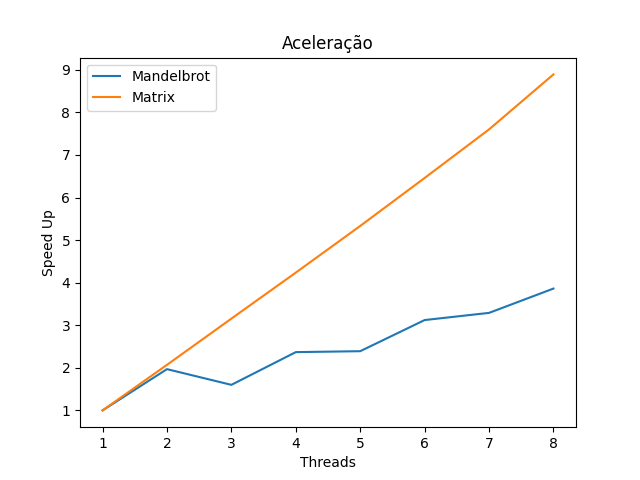
\includegraphics[scale=.7]{SpeedUp.png}

		É possível observar que o algoritmo de Mandelbrot não teve bom desempenho ao ser paralelizado, apesar de 
		ter um aumento de performance significativo em uma execução com 8 threads se comparada com a execução sequencial, 
		esse aumento não é tão grande se comparado com uma execução com apenas 6 threads. Mais ainda, o desempenho não é consistente, isto é,
		houveram situações onde execuções com menos threads tiveram desempenho melhor que execuções com mais threads.

		Já no caso do algoritmo de Multiplicação de Matrizes, temos um caso ideal, onde o desempenho do programa cresce linearmente
		com o aumento do número de threads utilizadas.

		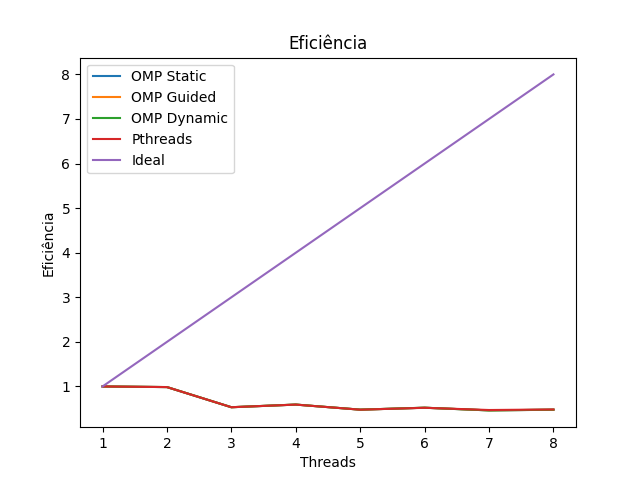
\includegraphics[scale=.7]{Eficiência.png}
		
		O algoritmo de Mandelbrot novamente teve um desempenho ruim. O gráfico torna evidente
		que este algoritmo, na sua implementação testada, não lida bem com paralelização além de duas threads.
		A baixa eficiência do algoritmo nos casos com mais de duas threads pode ser interpretada como uma indicação que
		a implementação de paralelismo testada não é a ideal e pode ser melhorada.

		Já o algoritmo de Multiplicação de Matrizes teve um desempenho peculiar. Ao contrário do algoritmo de Mandelbrot, sua
		eficiência continuamente aumentou com a adição de novas threads, não só isso, mas ela esteve acima de 100\% em todo os
		momentos, o que pode ser um indicador de que a implementação, no computador onde foi testada, tem comportamento superlinear.


\end{document}